\chapter{Implementation}\label{ch:implementation}

Following the design presented in the previous \cref{ch:design}, this chapter lays out the implementation of the system and the integration of the components that compose it, as well as the methodologies and tools used to develop, assemble, and integrate the system. As previously explained, the system is divided into four main components: the \gls{uav}, the control station, the reconnaissance platform, and the communication system. Each component is implemented separately and then integrated into the system as a whole following the V-model methodology described in \cref{ch:methodology_approach}.

\section{Unmanned Aerial Vehicle}\label{sec:implementation_uav}

The \gls{uav} is the base platform and the main component of the system. For this reason, it is the first component to be implemented. The \gls{uav} is responsible for carrying the reconnaissance platform and the communication system, as well as for executing the flight plan generated by the control station. The detailed implementation of the \gls{uav} is out of the scope of this thesis and only a high-level overview of the implementation is provided. However, more information about the implementation of the \gls{uav} can be found in the \autocite{developingcosteffectivedrones5g}. Each subsystem of the \gls{uav} described in the \cref{sec:design_uav}
is implemented separately and then integrated into the \gls{uav} as a whole.

\subsection{Airframe}\label{subsec:implementation_airframe}

For the airframe, the \gls{uav} was built using following the instructions provided by the manufacturer. The airframe can be seen in \cref{fig:airframe}. However, some modifications were made to the airframe to accommodate the additional components using custom 3D printed parts (e.g., the landing gear, the camera mount, and the payload bay). The design and manufacture of the 3D printed parts where made using the FreeCAD software \autocite{freecadFreeCADYour} and a Bamboo P1S 3D printer \autocite{bambulabBambuPrinter}. The reason to use 3D printed parts is that they are easy to design and manufacture, as well as being lightweight and durable. The 3D printed parts were designed to be easily attached to the airframe using screws and nuts, as well as to be easily removed in case of maintenance or replacement. Some of the 3D printed parts used in the airframe can be seen in \cref{fig:3d_printed_landing_gear_stl}.

\begin{figure}
  \begin{subfigure}{0.4\textwidth}
    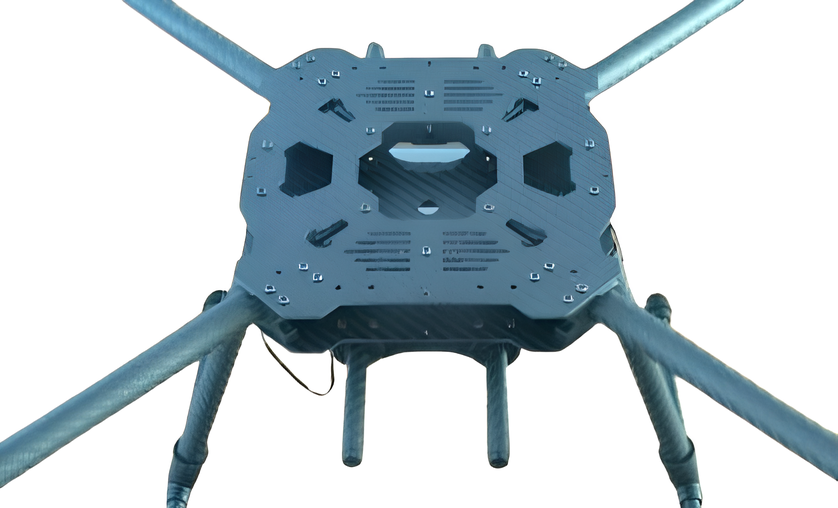
\includegraphics{airframe_tarot.png}
    \caption{Tarot XS690 airframe \autocite{developingcosteffectivedrones5g}.}\label{fig:airframe}
  \end{subfigure}
  \hfill
  \begin{subfigure}{0.4\textwidth}
    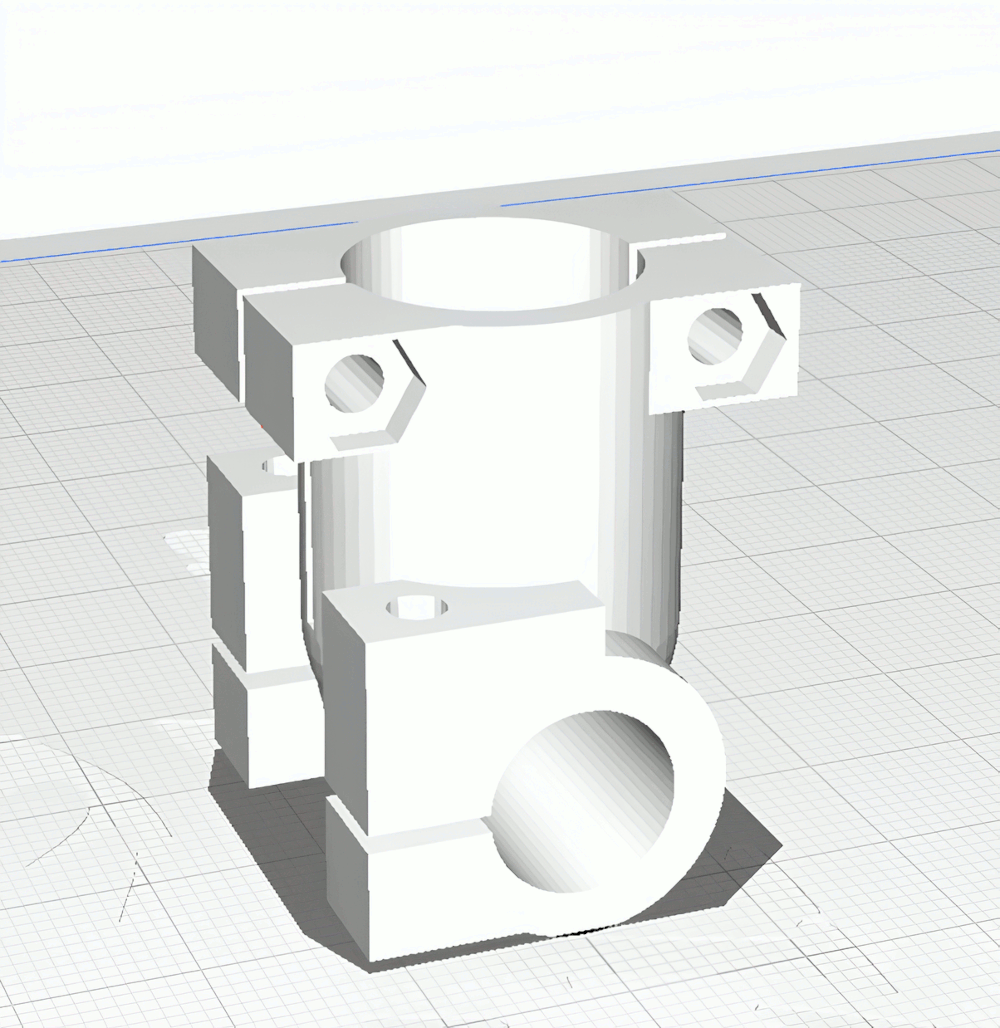
\includegraphics{3d_printed_landing_gear_stl.png}
    \caption{3D printed landing gear \autocite{developingcosteffectivedrones5g}.}\label{fig:3d_printed_landing_gear_stl}
  \end{subfigure}

  \caption{Airframe and 3D printed parts.}\label{fig:airframe_and_3d_printed_parts}
\end{figure}

\subsection{Propulsion System}\label{subsec:implementation_propulsion_system}

Regarding the propulsion system, the four motors were attached to the airframe using custom metal brackets, as seen in \cref{fig:motors_attached_to_airframe}. The \glspl{esc} were attached to the airframe using double-sided tape and zip ties, as seen in \cref{fig:esc_attached_to_airframe}.

\begin{figure}
  \hfill
  \begin{subfigure}{0.4\textwidth}
    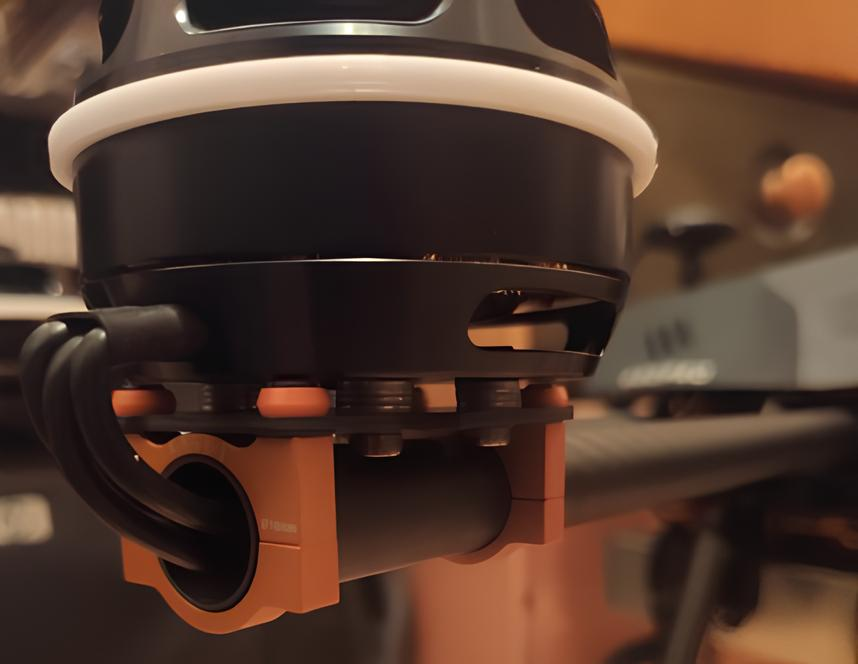
\includegraphics{motor_mount.jpg}
    \caption{Metal motor mount brackets to attach the motors to the airframe (orange brackets) \autocite{developingcosteffectivedrones5g}.}\label{fig:motors_attached_to_airframe}
  \end{subfigure}
  \hfill
  \begin{subfigure}{0.4\textwidth}
    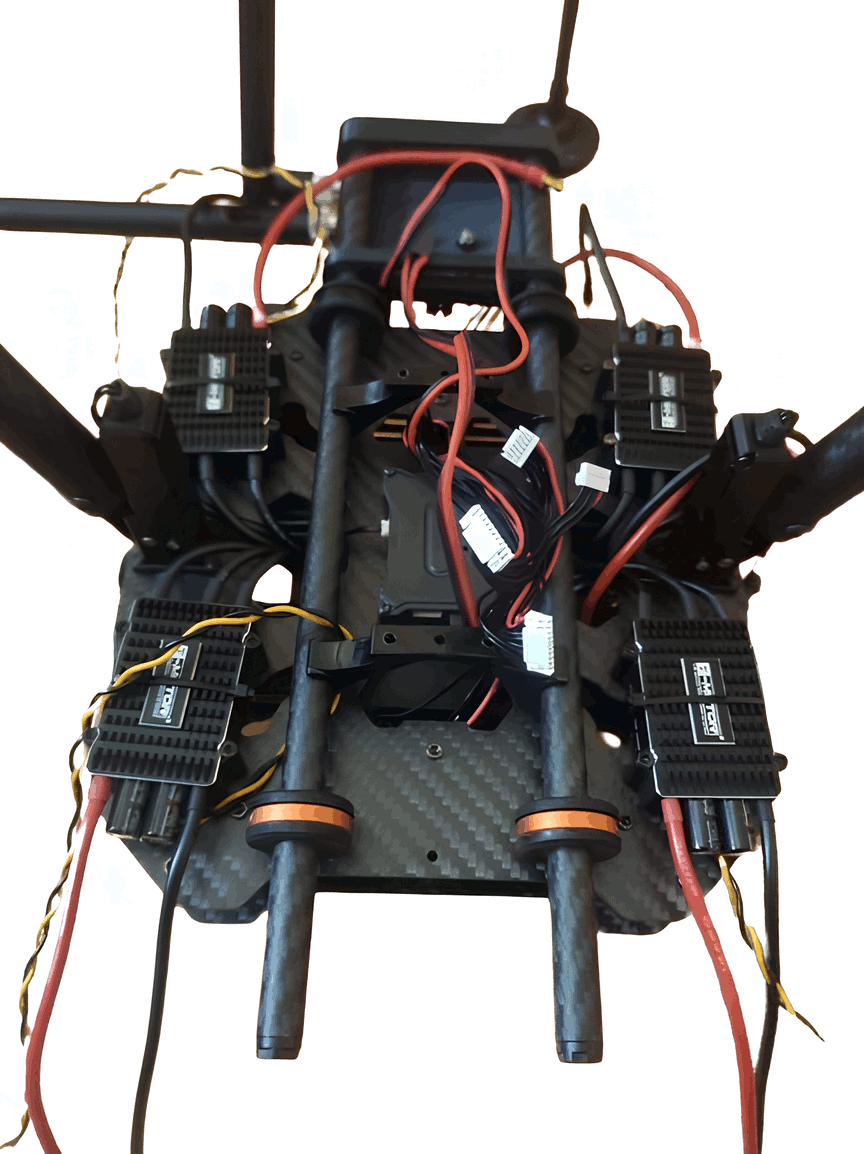
\includegraphics{bottom_plate_esc.png}
    \caption{Bottom view of the airframe with the \glspl{esc} attached in each corner \autocite{developingcosteffectivedrones5g}.}\label{fig:esc_attached_to_airframe}
  \end{subfigure}
  \hfill

  \caption{Propulsion system components attached to the airframe.}\label{fig:propulsion_system_components_attached_to_airframe}
\end{figure}

\subsection{Flight Controller}\label{subsec:implementation_flight_controller}

For the flight controller, it was placed in the middle of the airframe using double-sided tape and zip ties, as seen in \cref{fig:flight_controller_attached_to_airframe}. It is important to note that placing the flight controller in the middle of the airframe provides the best balance and stability for the \gls{uav} during flight.

\begin{figure}
  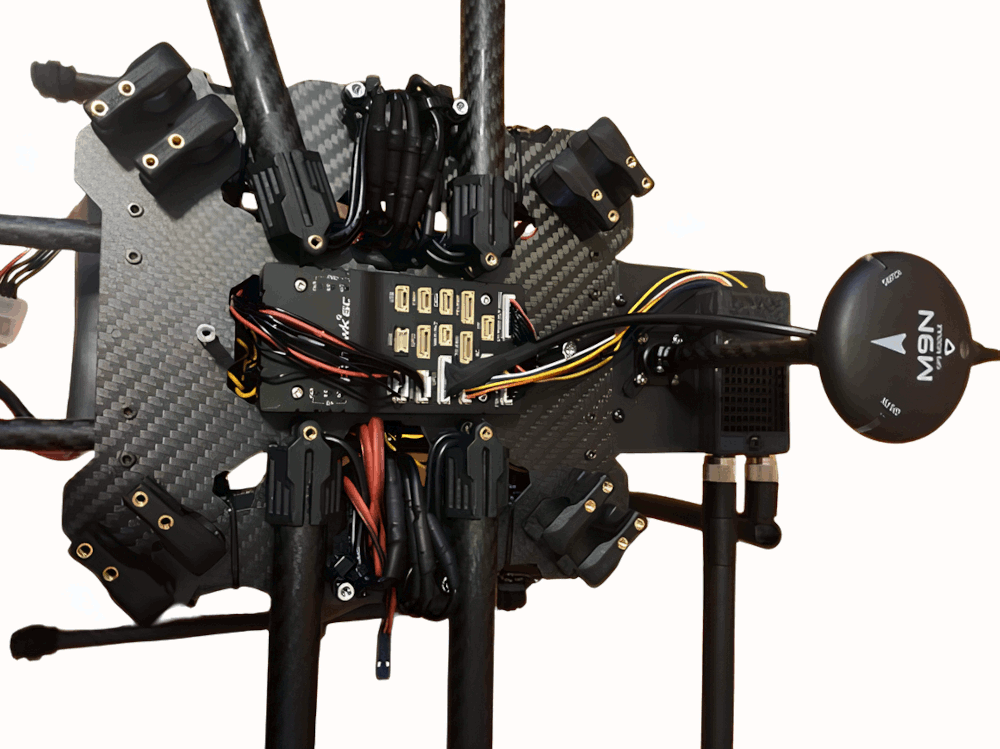
\includegraphics[width=0.4\textwidth]{mid_plate_flight_controller.png}
  \caption{Flight controller attached to the airframe in the middle of the airframe \autocite{developingcosteffectivedrones5g}.}\label{fig:flight_controller_attached_to_airframe}
\end{figure}

\subsection{Power System}\label{subsec:implementation_power_system}

The power system is the heaviest subsystem of the \gls{uav} and must be placed in the center of the airframe to provide the best balance and stability during flight. The battery was attached to the airframe using battery straps, as seen in \cref{fig:battery_attached_to_airframe}. The \gls{pdb}, \cref{fig:pdb}, was attached to the airframe using a custom 3D printed mount and places in the middle of the airframe, as seen in \cref{fig:power_distribution_board_attached_to_airframe}. Also, the voltage regulator was attached to the top of the airframe using double-sided tape and zip ties, refer to \cref{fig:computer_attached_to_airframe}.

\begin{figure}
  \hfill
  \begin{subfigure}[t]{0.3\linewidth}
    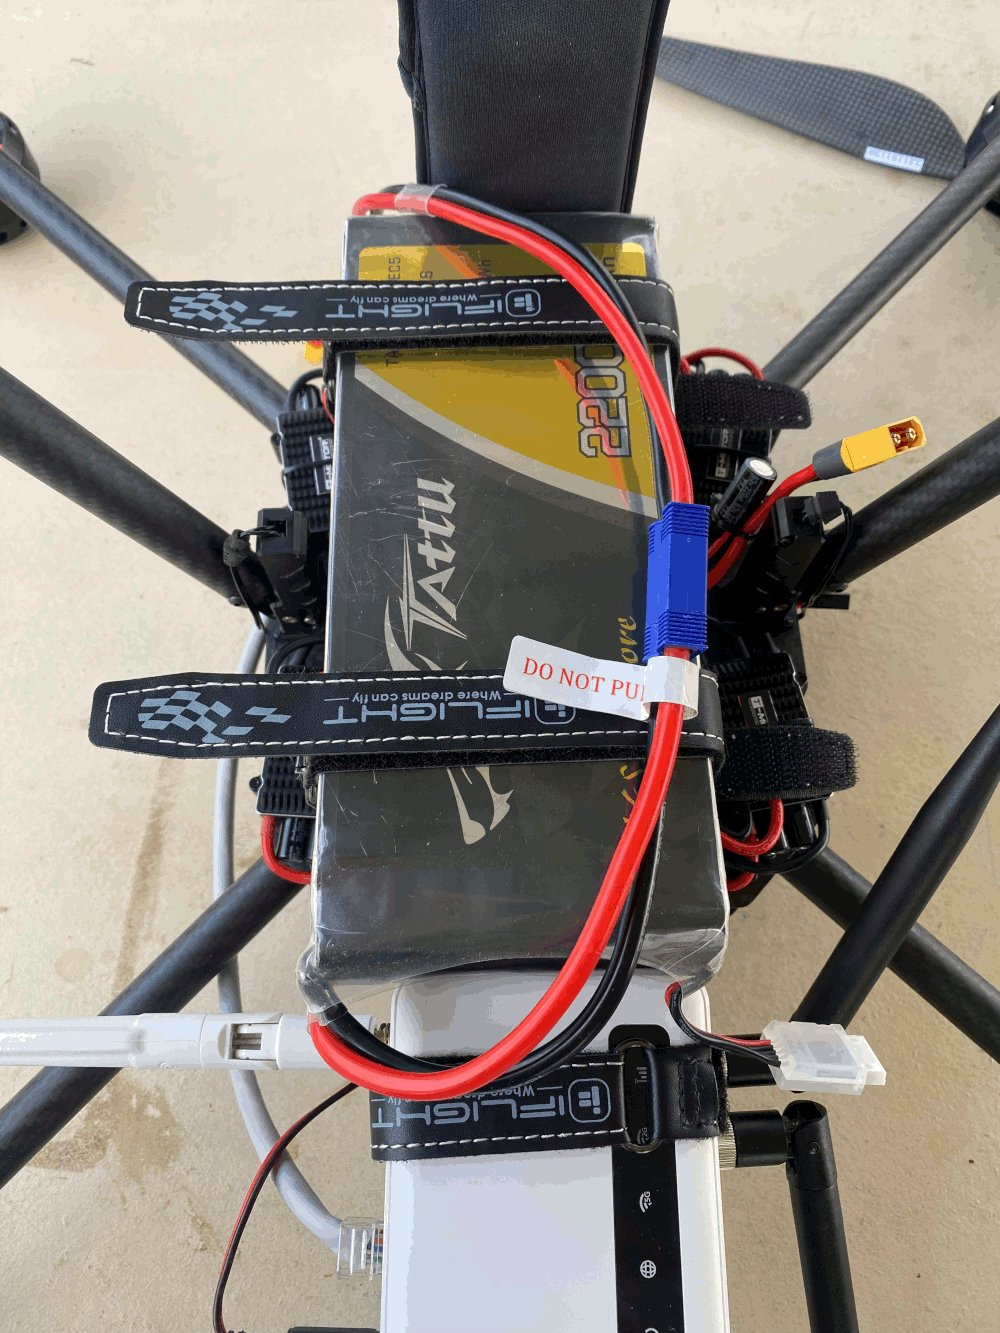
\includegraphics[width=\linewidth]{bottom_plate_battery.jpg}
    \caption{Battery attached to the airframe.}\label{fig:battery_attached_to_airframe}
  \end{subfigure}
  \hfill
  \begin{subfigure}[t]{0.3\linewidth}
    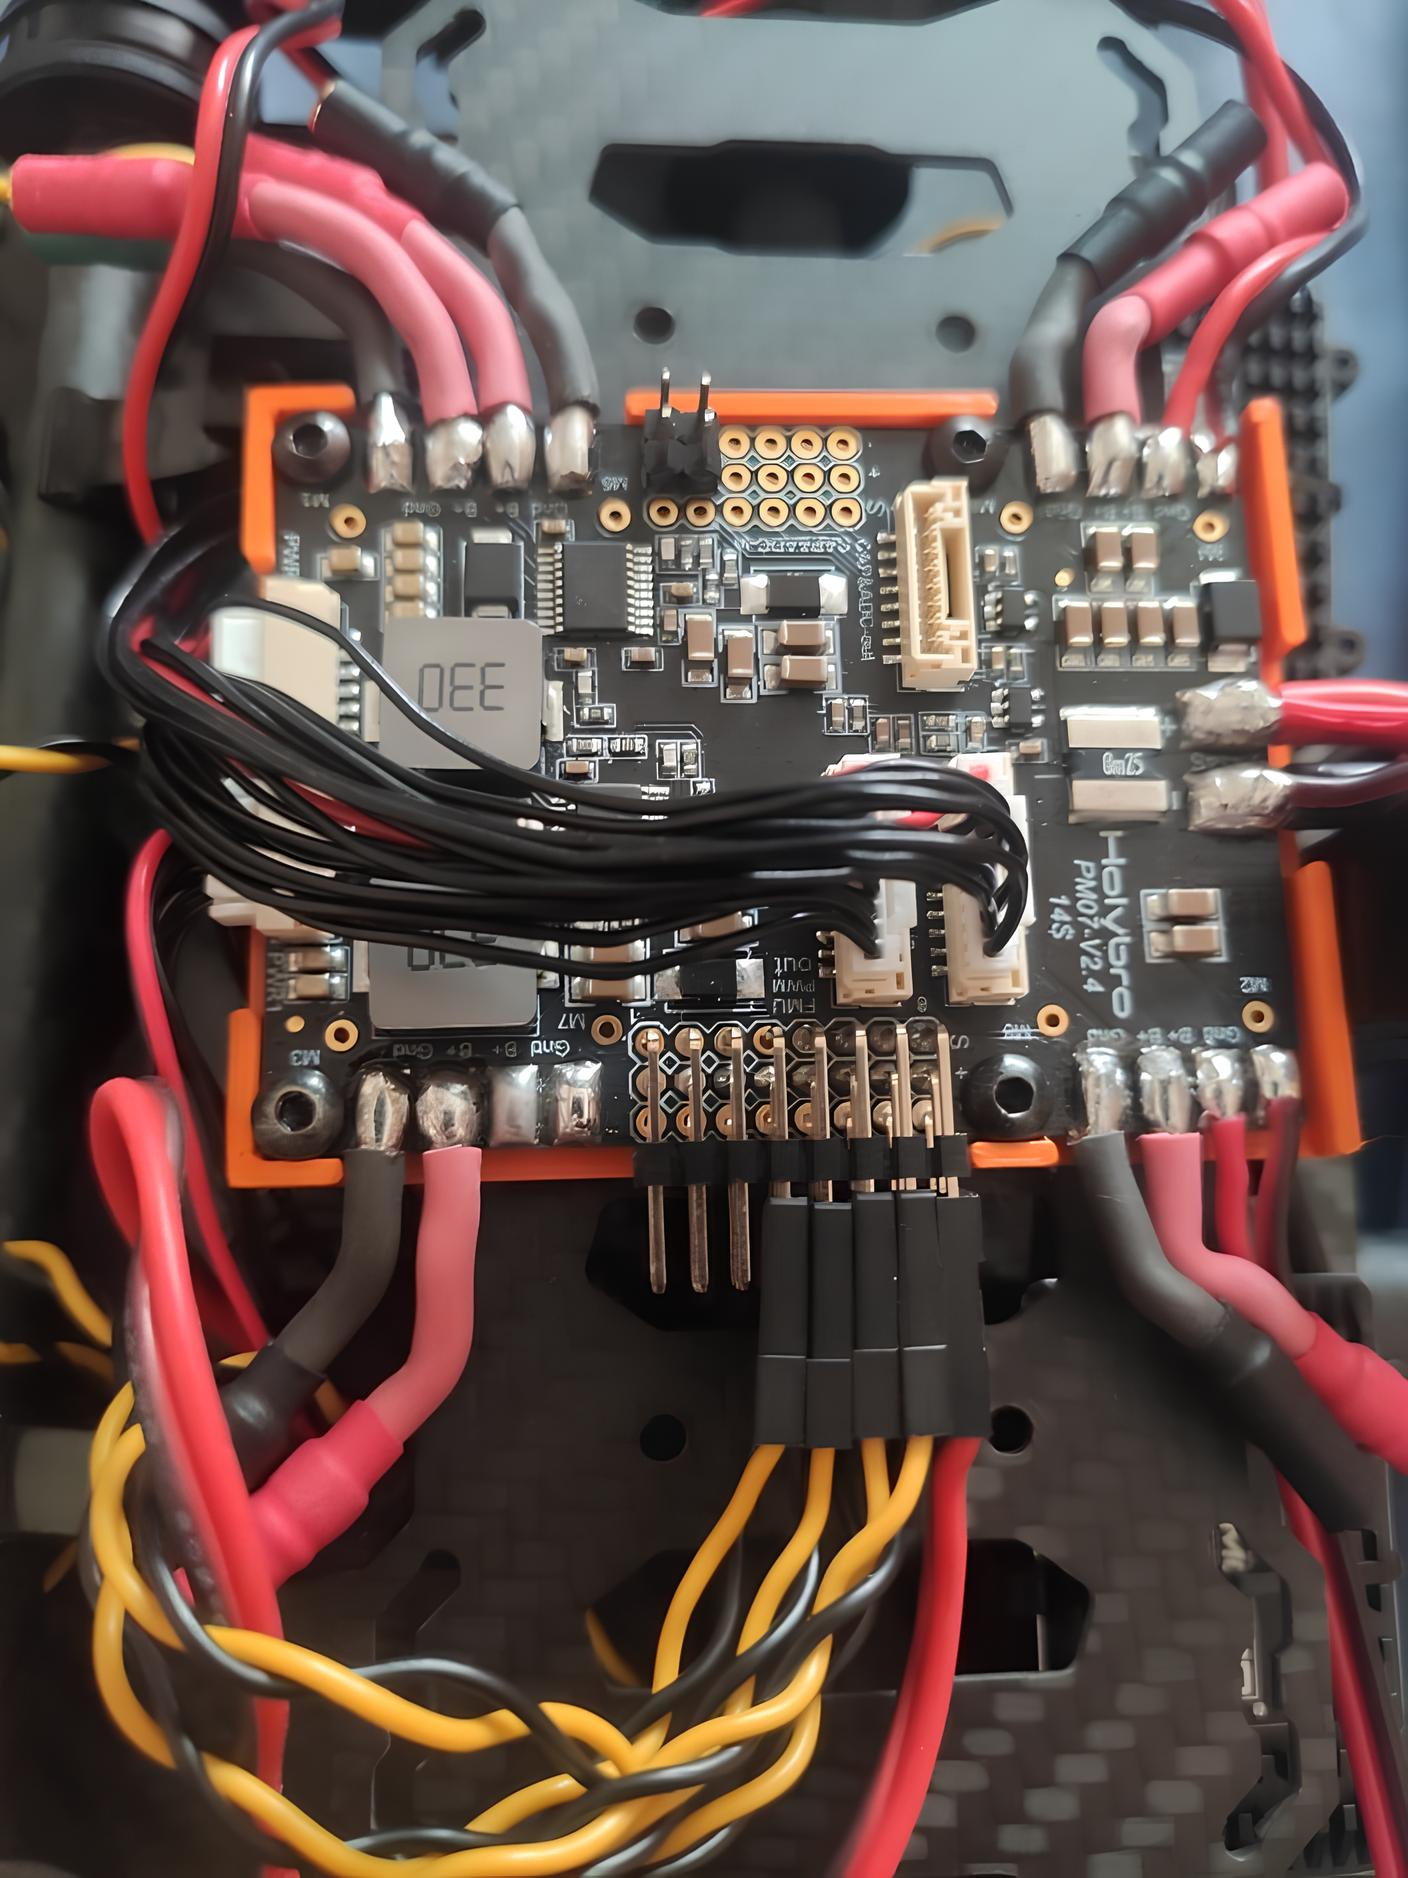
\includegraphics[width=\linewidth]{mid_plate_pdb.jpg}
    \caption{\gls{pdb} attached to the mid plate of the airframe \autocite{developingcosteffectivedrones5g}.}\label{fig:pdb}
  \end{subfigure}
  \hfill
  \begin{subfigure}[t]{0.3\linewidth}
    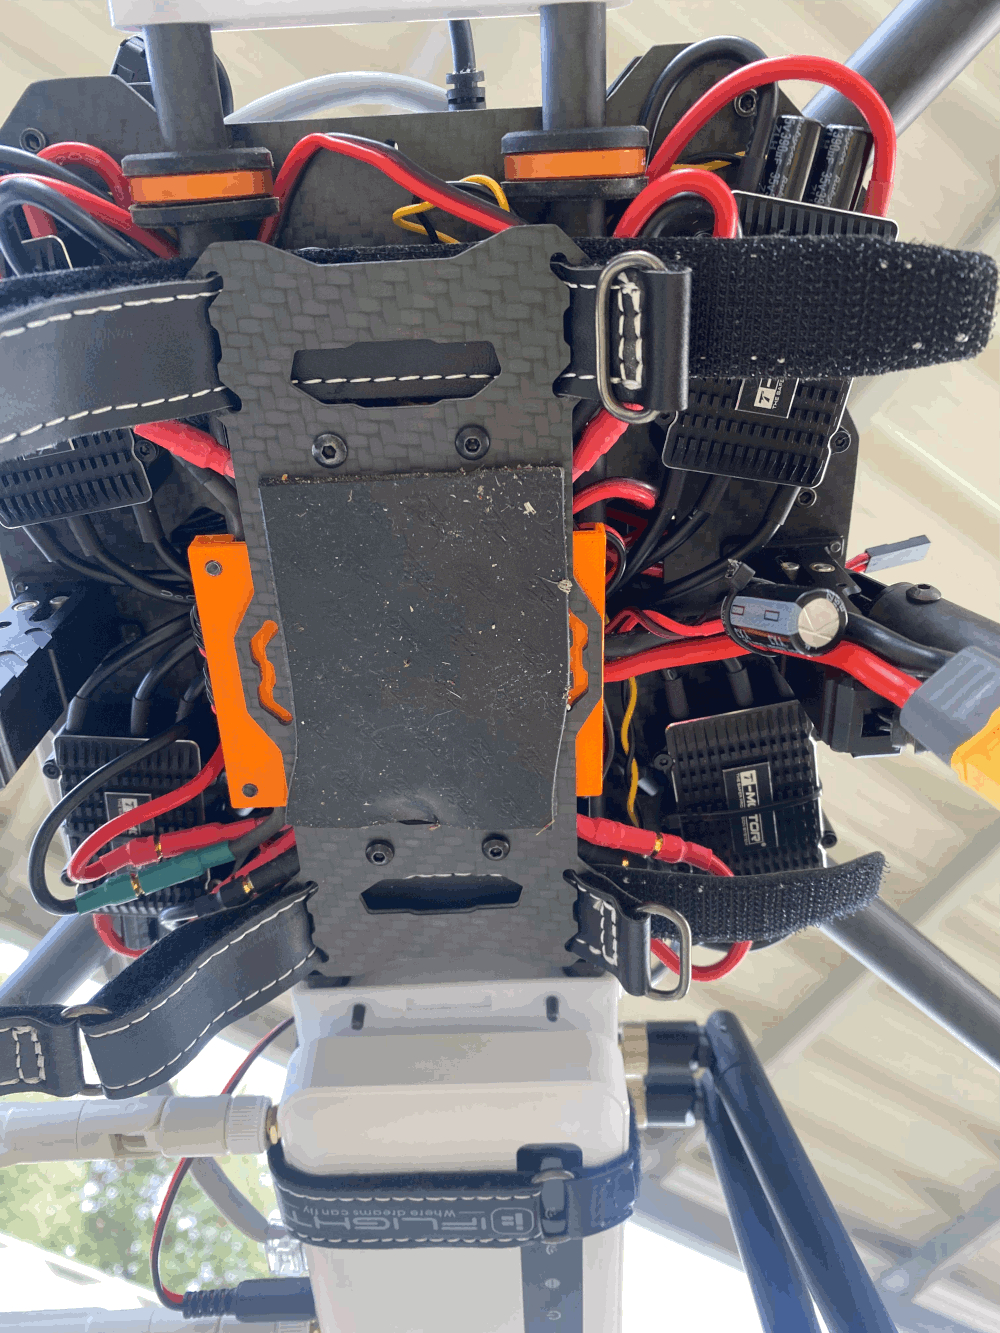
\includegraphics[width=\linewidth]{mid_plate_pdb_mounted.jpg}
    \caption{\gls{pdb} attached to the airframe, orange box in the middle of the airframe.}\label{fig:power_distribution_board_attached_to_airframe}
  \end{subfigure}
  \hfill

  \caption{Power system components attached to the airframe.}\label{fig:power_system_components_attached_to_airframe}
\end{figure}

\subsection{Peripherals}\label{subsec:implementation_peripherals}

The \gls{gps} was attached to the top of the airframe using a custom 3D printed mount, as seen in \cref{fig:gps_attached_to_airframe}. A important note is that the \gls{gps} module must be placed in a location where it has the best reception, as well as where it is not obstructed by other components of the \gls{uav}. It must be place as far as possible from the motors and any carbon fiber components, as they can interfere with the reception of the \gls{gps} module.

For the communication system, the \gls{rf} module was attached to the airframe using the same 3D printed mount as the \gls{gps} module, as seen in \cref{fig:gps_attached_to_airframe}. The \gls{4g} module was attached to the airframe along with the \gls{rf} module and the \gls{gps} module.

The camera was attached to the front of the airframe using a custom 3D printed mount in order to provide the best \gls{fov}, as seen in \cref{fig:camera_attached_to_airframe}. The camera must be placed in a location where it has the best field of view, as well as where it is not obstructed by other components of the \gls{uav}. It must be placed as far as possible from the motors as they can interfere with the camera's \gls{fov}.

Finally, for the on-board computer, it was placed in the middle of the airframe using screws and nuts, as seen in \cref{fig:computer_attached_to_airframe}. It must be placed in a location where air can flow freely to avoid overheating. Depending on the application, the on-board computer can be placed in a different location, as long as it is not obstructed by other components of the \gls{uav}, however, it is recommended to place it in the middle of the airframe to provide the best balance and stability during flight.

\begin{figure}
  \hfill
  \begin{subfigure}[t]{0.3\linewidth}
    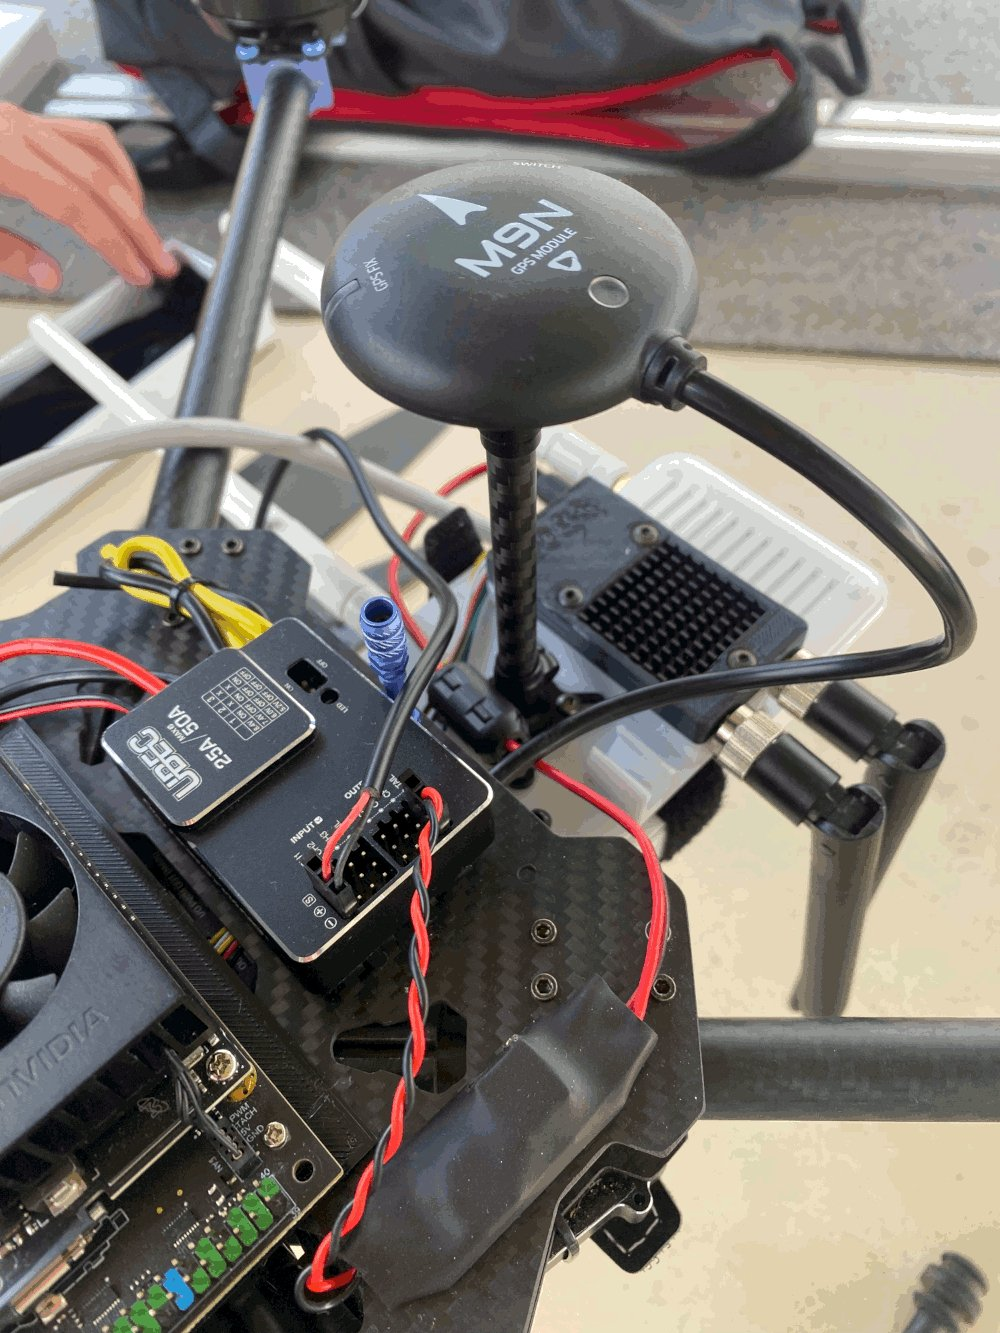
\includegraphics[width=\linewidth]{top_plate_gps.jpg}
    \caption{\gls{gps} module attached to the airframe (circular black module). The \gls{rf} module is the rectangular black module with two antennas behind the \gls{gps} module. The \gls{4g} router is the white module below the \gls{rf} module.}\label{fig:gps_attached_to_airframe}
  \end{subfigure}
  \hfill
  \begin{subfigure}[t]{0.3\linewidth}
    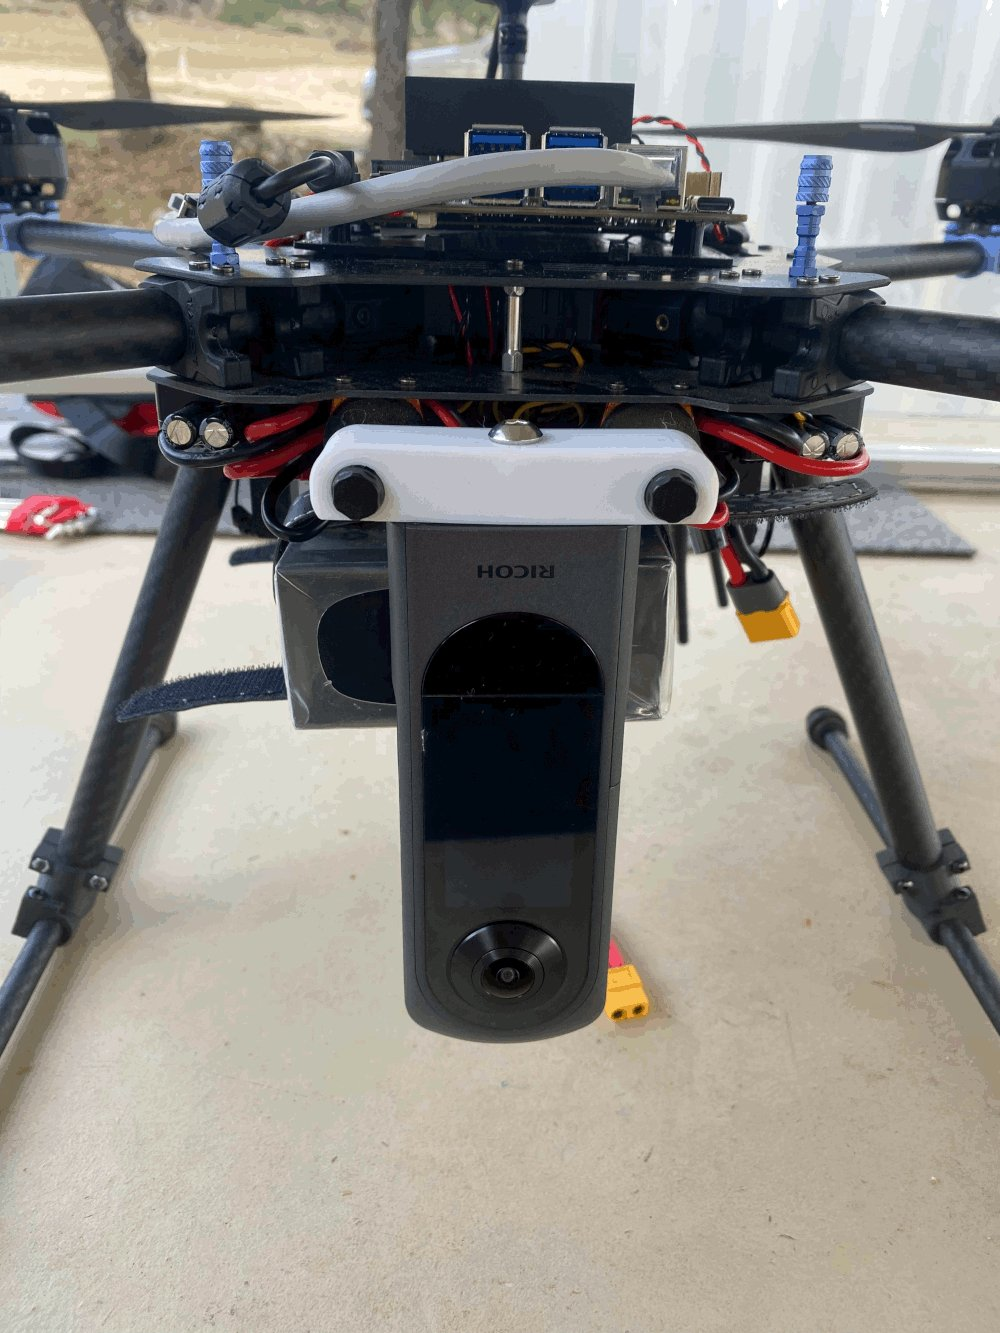
\includegraphics[width=\linewidth]{front_mount_camera.jpg}
    \caption{Camera attached to the airframe using a custom 3D printed white mount.}\label{fig:camera_attached_to_airframe}
  \end{subfigure}
  \hfill
  \begin{subfigure}[t]{0.3\linewidth}
    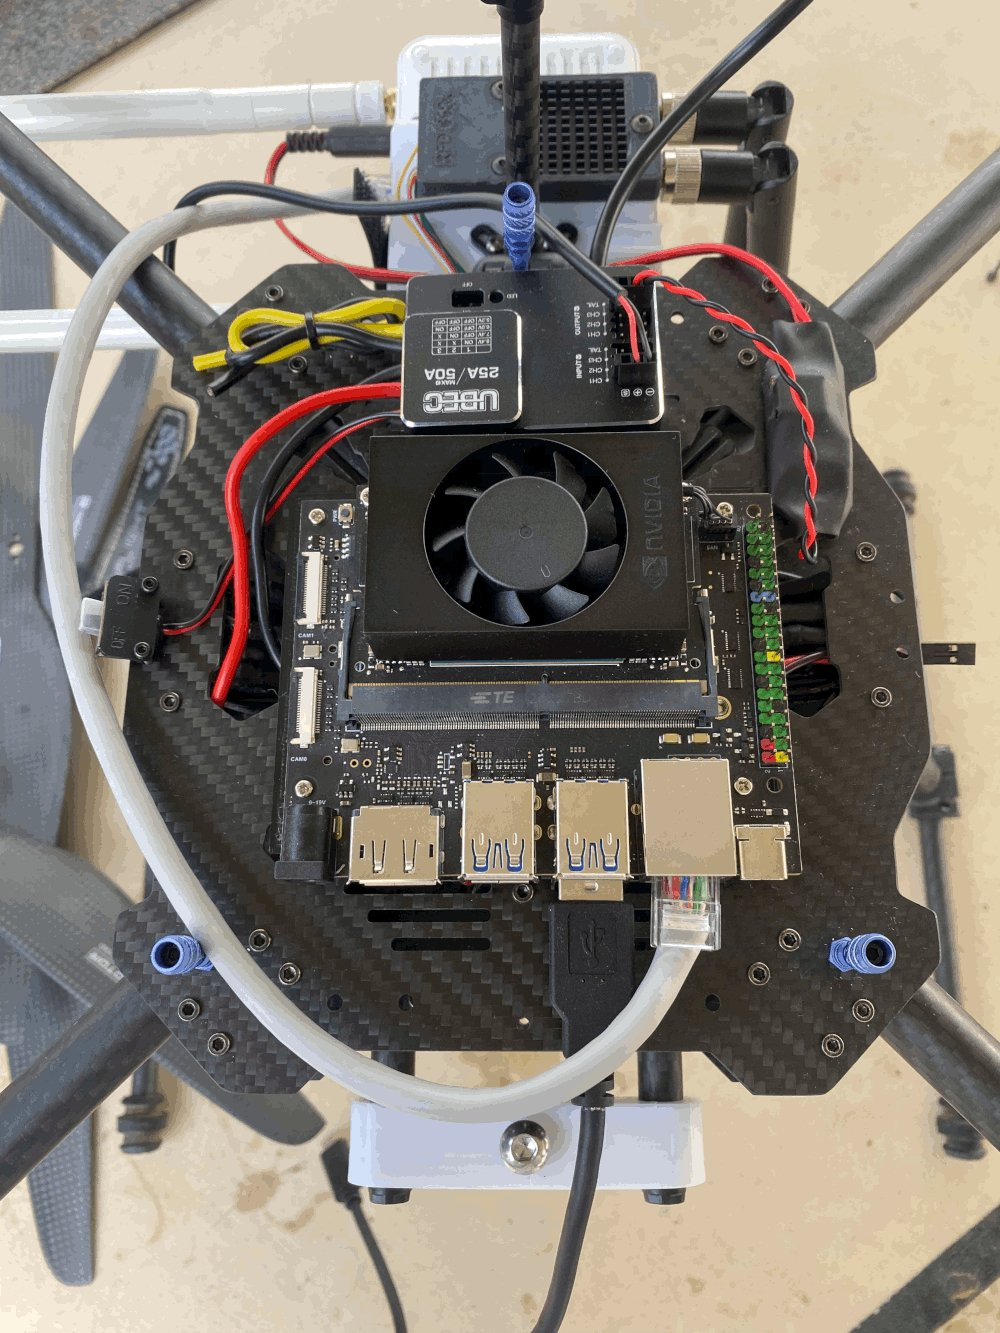
\includegraphics[width=\linewidth]{top_mount_computer.jpg}
    \caption{On the center, the on-board computer. On the top side above the fan, the \gls{gps} module.}\label{fig:computer_attached_to_airframe}
  \end{subfigure}
  \hfill

  \caption{Peripherals attached to the airframe.}\label{fig:peripherals_attached_to_airframe}
\end{figure}

\subsection{Final Assembly}\label{subsec:implementation_final_assembly}

After all the components were attached to the airframe, the final assembly of the \gls{uav} was performed. The final assembly consists of connecting all the components together, as well as configuring the flight controller and the communication system. The final assembly of the \gls{uav} can be seen in \cref{fig:uav_assembled}.

\begin{figure}
  \hfill
  \begin{subfigure}[t]{0.4\linewidth}
    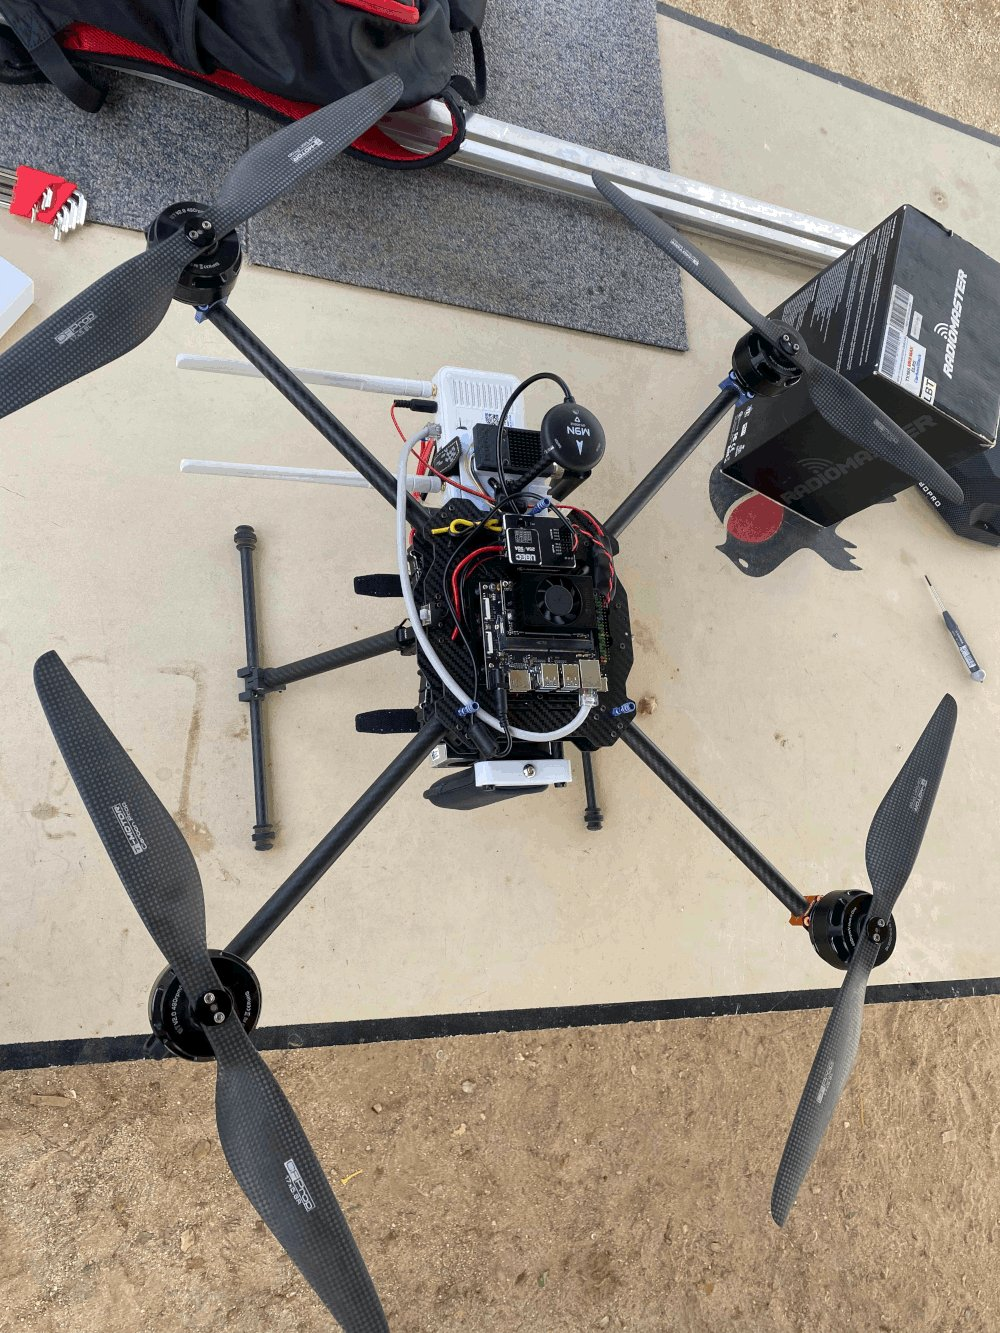
\includegraphics[width=\linewidth]{final_assembly_top.jpg}
    \caption{Top view of the \gls{uav} assembled.}\label{fig:uav_assembled_top}
  \end{subfigure}
  \hfill
  \begin{subfigure}[t]{0.4\linewidth}
    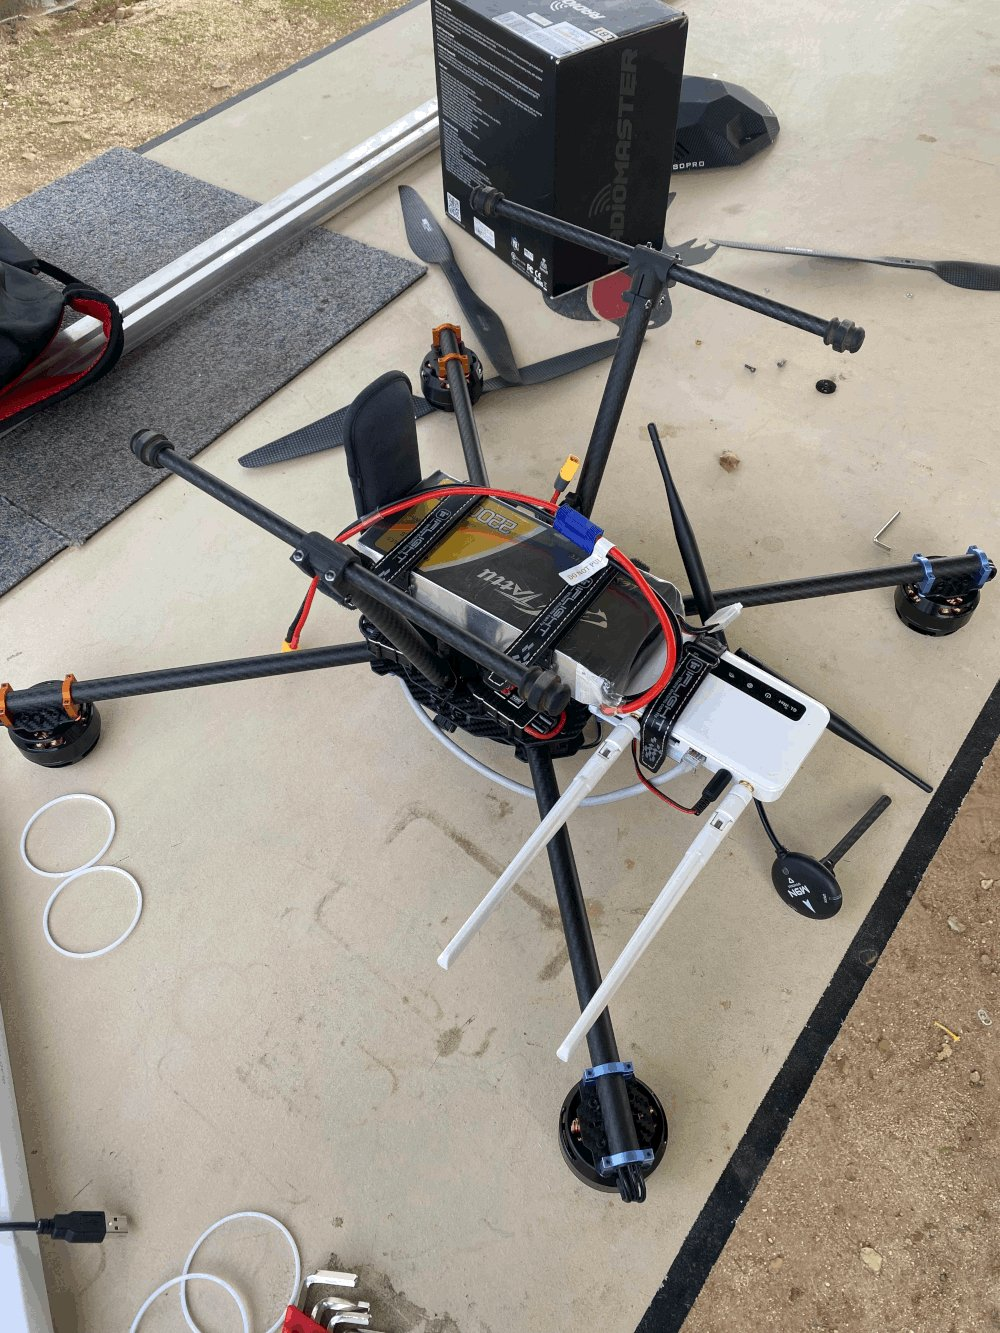
\includegraphics[width=\linewidth]{final_assembly_bottom.jpg}
    \caption{Bottom view of the \gls{uav} assembled.}\label{fig:uav_assembled_bottom}
  \end{subfigure}
  \hfill

  \caption{Final assembly of the \gls{uav}.}\label{fig:uav_assembled}
\end{figure}

\section{Control Station}\label{sec:implementation_control_station}

\section{Communication System}\label{sec:implementation_communication_system}

\section{Reconnaissance Platform}\label{sec:implementation_reconnaissance_platform}

Finally, to implement the reconnaissance platform, three main components are needed: video capture, video processing, and insights generation. The video capture component is responsible for capturing the video feed from the \gls{uav} camera. The video processing component is responsible for processing the video feed to extract relevant information. The insights generation component is responsible for generating insights from the processed video feed. Each different component is implemented separately and then integrated into the reconnaissance platform as a whole.

\subsection{Video Capture}\label{subsec:implementation_video_capture}

In order to capture the video from the Ricoh Theta X 360 Degree Camera \autocite{ricohimagingTHETARicoh}, the camera is connected to the NVIDIA Jetson Orin \autocite{nvidiaNVIDIAJetson} using a \gls{usb} C cable. The camera is configured to stream the video feed to the NVIDIA Jetson Orin using the Ricoh Theta X 360 Degree Camera API \autocite{ricoh360ReferenceRicoh}. In order to be able to capture the video feed from the camera, several libraries are used, such as OpenCV \autocite{githubGitHubOpencvopencv}, GSTThetaUVC \autocite{githubGitHubBuburidergstthetauvc}, LibUVC \autocite{githubGitHub6GIntegration3UC3Mlibuvcthetasample}, and V4L2 \autocite{githubGitHubUmlaeutev4l2loopback}. It is worth mentioning that the libraries used had to be modified to work with the Ricoh Theta X 360 Degree Camera, as it is not officially supported by the libraries. The video feed is captured in real-time and sent to the video processing component for further processing.

\subsection{Video Processing}\label{subsec:implementation_video_processing}

Once the video feed is captured by the Jetson Orin, it is further processed to extract relevant information. The video processing is done using deep learning algorithms to detect and track objects in the environment. The model used for the object detection and tracking is the YOLOv11 \autocite{ultralyticsYOLO11} as it is the defacto standard for object detection and tracking in real-time. It provides the best performance in terms of accuracy and speed, as well as being able to run on the Jetson Orin. The model used was the YOLOv11-medium with a pixel resolution of 640x640 px and an inference time of \SI{56}{\milli\second}. In \cref{fig:drone_yolo_detection}, an example of the video feed captured by the camera can be seen, note a single frame is showcased.

\begin{figure}
	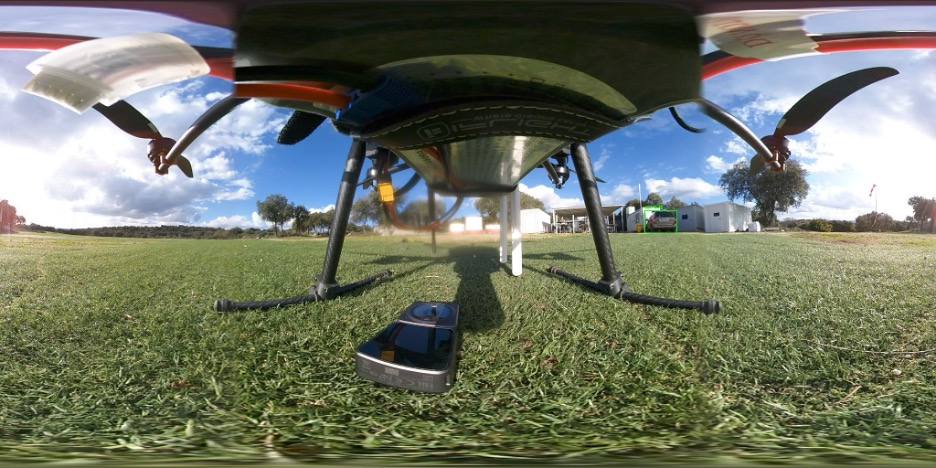
\includegraphics[]{drone_yolo_detection.jpg}
	\caption{Detection example of the video processing with a YOLOv11. The green box  on the middle right side of the image corresponds to the bounding box of the car.}\label{fig:drone_yolo_detection}
\end{figure}

\subsection{Insights Generation}\label{subsec:implementation_insights_generation}

Finally, all the detected and tracked objects are sent to the insights generation component to generate insights for the end-user. In order to process the detected and tracked objects, a web application was developed using the NextJS framework \autocite{nextjsNextjsVercel}. This web application is responsible for displaying the detected and tracked objects in real-time, as well as generating alerts and notifications in case of critical events or failures. The web application is also responsible for managing the different missions of the \glspl{uav} with the objectives and constraints defined by the end-user and also handling the user authentication and authorization.

The web application is divided into three main layers: the presentation layer, the application layer, and the data layer. The application layer is responsible for handling the business logic of the web application, such as the user authentication and authorization, the mission management, the rule management, the detection management, the alert management, and the notification management. The presentation layer is responsible for displaying the information to the end-user. The data layer is responsible for storing the information of the web application.

\subsubsection{Presentation Layer}\label{subsubsec:implementation_presentation_layer}

The presentation layer is developed using the ReactJS framework \autocite{reactReact} for the frontend, Tailwind CSS \autocite{tailwindcssTailwindRapidly} for the styling, and Prisma \autocite{prismaPrismaSimplify} for the database handling. In order to provide a responsive and user-friendly interface, the web application is divided into different components, such as the login component, the dashboard component, the mission component, the drone component. Each component is responsible for displaying the information to the end-user and providing the necessary functionalities to interact with the system. The web application is designed to be easy to use and intuitive, as well as to provide real-time updates and notifications to the end-user. In \cref{fig:web_application}, a screenshot of the web application can be seen.

\begin{figure}
	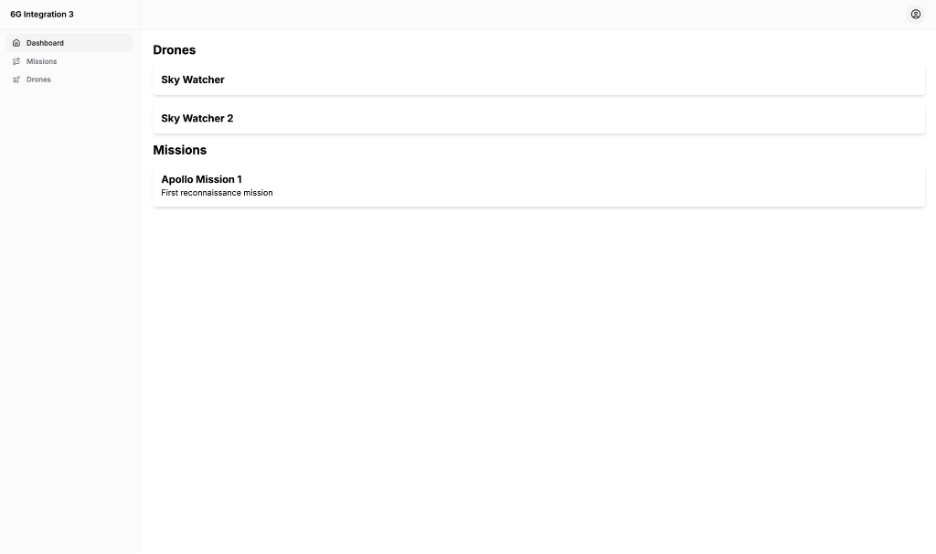
\includegraphics[]{website_showcase.png}
	\caption{Screenshot of the web application showcasing the dashboard.}\label{fig:web_application}
\end{figure}

\subsubsection{Data Layer}\label{subsubsec:implementation_data_layer}

The data layers are divided into two main components: the object storage and the database. The object storage is used to store the video feed captured by the camera, as well as the detected and tracked objects. The object storage used was Amazon S3 \autocite{amazonCloudComputing}, as it provides a reliable and scalable storage solution for the web application.  For the database, a relational database was used to store the information of the web application. As Prisma \autocite{prismaPrismaSimplify} was used for the database handling, the database chosen can be any database supported by Prisma, such as PostgreSQL, MySQL, SQLite. This was chosen to provide flexibility and scalability to the system, as well as to be able to easily switch between databases if needed for different use cases such as testing, development, or production. The schema of the database can be seen in \cref{fig:database_schema}. The schema has six main tables, each one responsible for storing different information:

\begin{itemize}
	\item User: stores the information of the users of the system that can access the web application. It is used for user authentication and authorization purposes.

	\item Drone: stores the information of the drones that are connected to the system. It is used to manage the different drones and their missions. Each drone has a unique identifier, and a specific secret token to authenticate with the system and allow the drone to send the data to the system.

	\item Mission: stores the information of the missions of the drones. It is used to manage the different missions of the drones and group drones together for specific tasks. Each mission can be composed of one or more drones, and each drone can be part of one or more missions. Moreover, users are assigned to missions to have access to the data collected by the drones.

	\item Rule: stores the information of the rules of a specific mission to generate alerts and notifications. It is used to define the objectives and constraints of a mission, such as the specific objects to detect and track, the specific alerts to generate, and the specific notifications to send.

	\item Detection: stores the information of the detected objects in the environment by a drone for a specific mission. It is used to store the detected objects and their properties, such as the class, the confidence, the position, the size, and the orientation.

	\item Alert: stores the information of the alerts generated by the system for a specific mission created by a rule. It is used to store the alerts and their properties, such as the type, the severity, the message, the timestamp, and the status.
\end{itemize}

\begin{figure}
	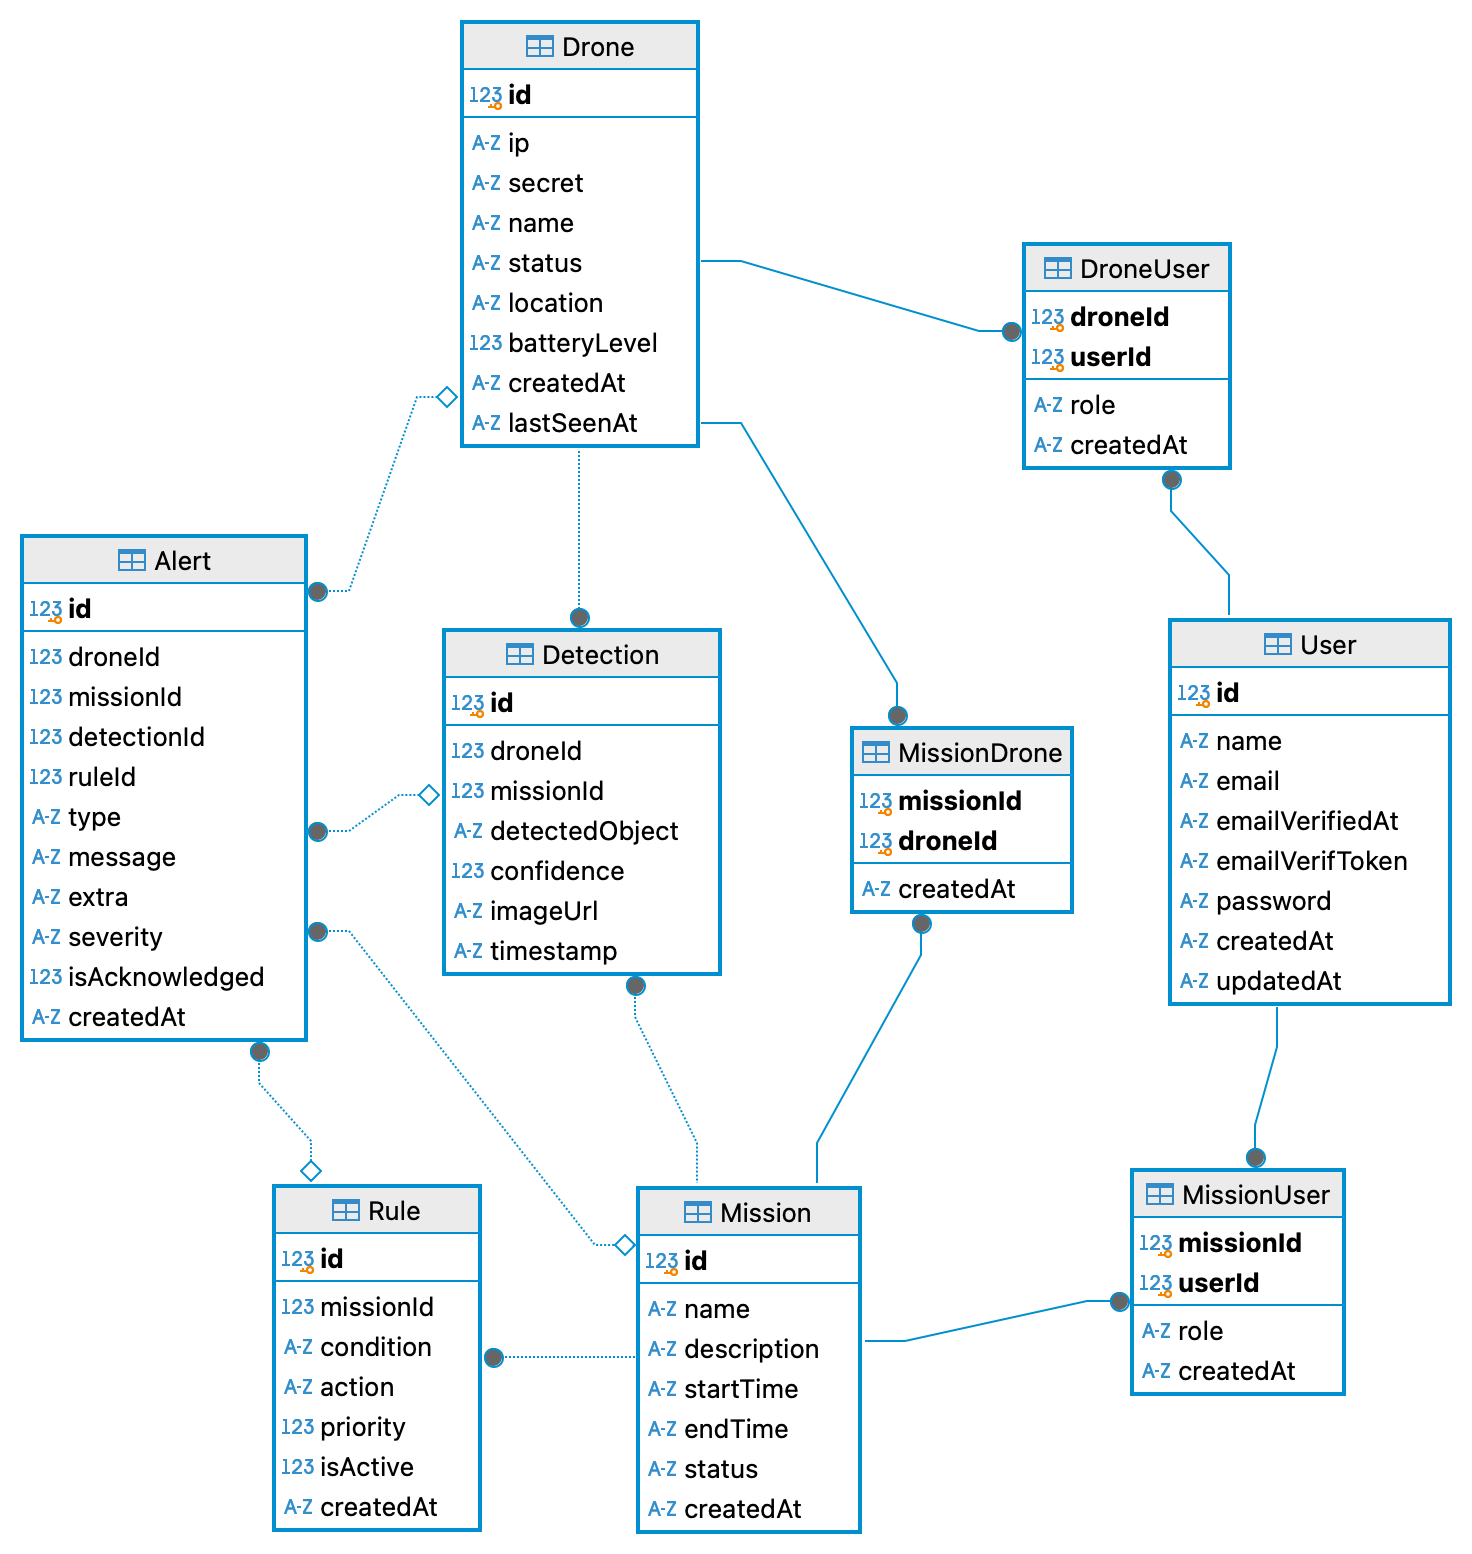
\includegraphics{reconnaissance_platform_database_schema.png}
	\caption{Database schema of the reconnaissance platform.}\label{fig:database_schema}
\end{figure}

\subsubsection{Application Layer}\label{subsubsec:implementation_application_layer}

The application layer forms the core of the web application, handling crucial business logic and system functionalities. This layer is responsible for managing various aspects of the reconnaissance platform, including:

\begin{itemize}
	\item User Authentication and Authorization: Implements secure login mechanisms and controls access to different parts of the system based on user roles and permissions. It is done with email password authentication and verification using the NextAuth.js library \autocite{nextauthNextAuthjsAuthentication}.

	\item Mission Management: Oversees the creation, modification, and execution of drone missions. This includes defining mission parameters, assigning drones, and monitoring mission progress.

	\item Rule Management: Allows users to set up and modify rules for generating alerts and notifications based on specific conditions or events detected during missions.

	\item Detection Management: Processes and organizes the data from detected and tracked objects, making it available for analysis and visualization.

	\item Alert Management: Generates and manages alerts based on predefined rules, ensuring that critical events are promptly communicated to relevant users.

	\item Notification Management: Handles the distribution of notifications to users through various channels, keeping them informed about mission status, alerts, and system updates.
\end{itemize}

The application layer serves as the intermediary between the presentation layer and the data layer, ensuring efficient data flow and processing. It implements the business logic that interprets user actions from the presentation layer, interacts with the data layer to retrieve or store information, and prepares the data for display in the user interface.

\subsubsection{LLM Integration}\label{subsubsec:implementation_llm_integration}

Moreover, the detected and tracked objects are further processed through an \gls{llm} integration, in this case Llama 3.2 11b Vision \autocite{llama3.211bvision}, using the Groq \glsentryshort{api} to extract additional contextual information and insights. This integration enhances the system's analytical capabilities by providing detailed descriptions, identifying potential relationships between detected objects, and generating natural language summaries of the surveillance data.

The \gls{llm} component receives the object detection data from the server with a specific prompt that the server operator wants to send and processes it to provide comprehensive analysis that includes object classification details, behavioral patterns, and potential security implications. This additional layer of intelligence helps operators make more informed decisions by providing context-rich information about the detected objects in real-time. The results from the \gls{llm} analysis are stored in the database and made available through the web interface, where they can be accessed alongside the original detection data and visual feeds.

In \cref{fig:llm_detection}, an example of the \gls{llm} detection results for a person can be seen.

\begin{figure}
	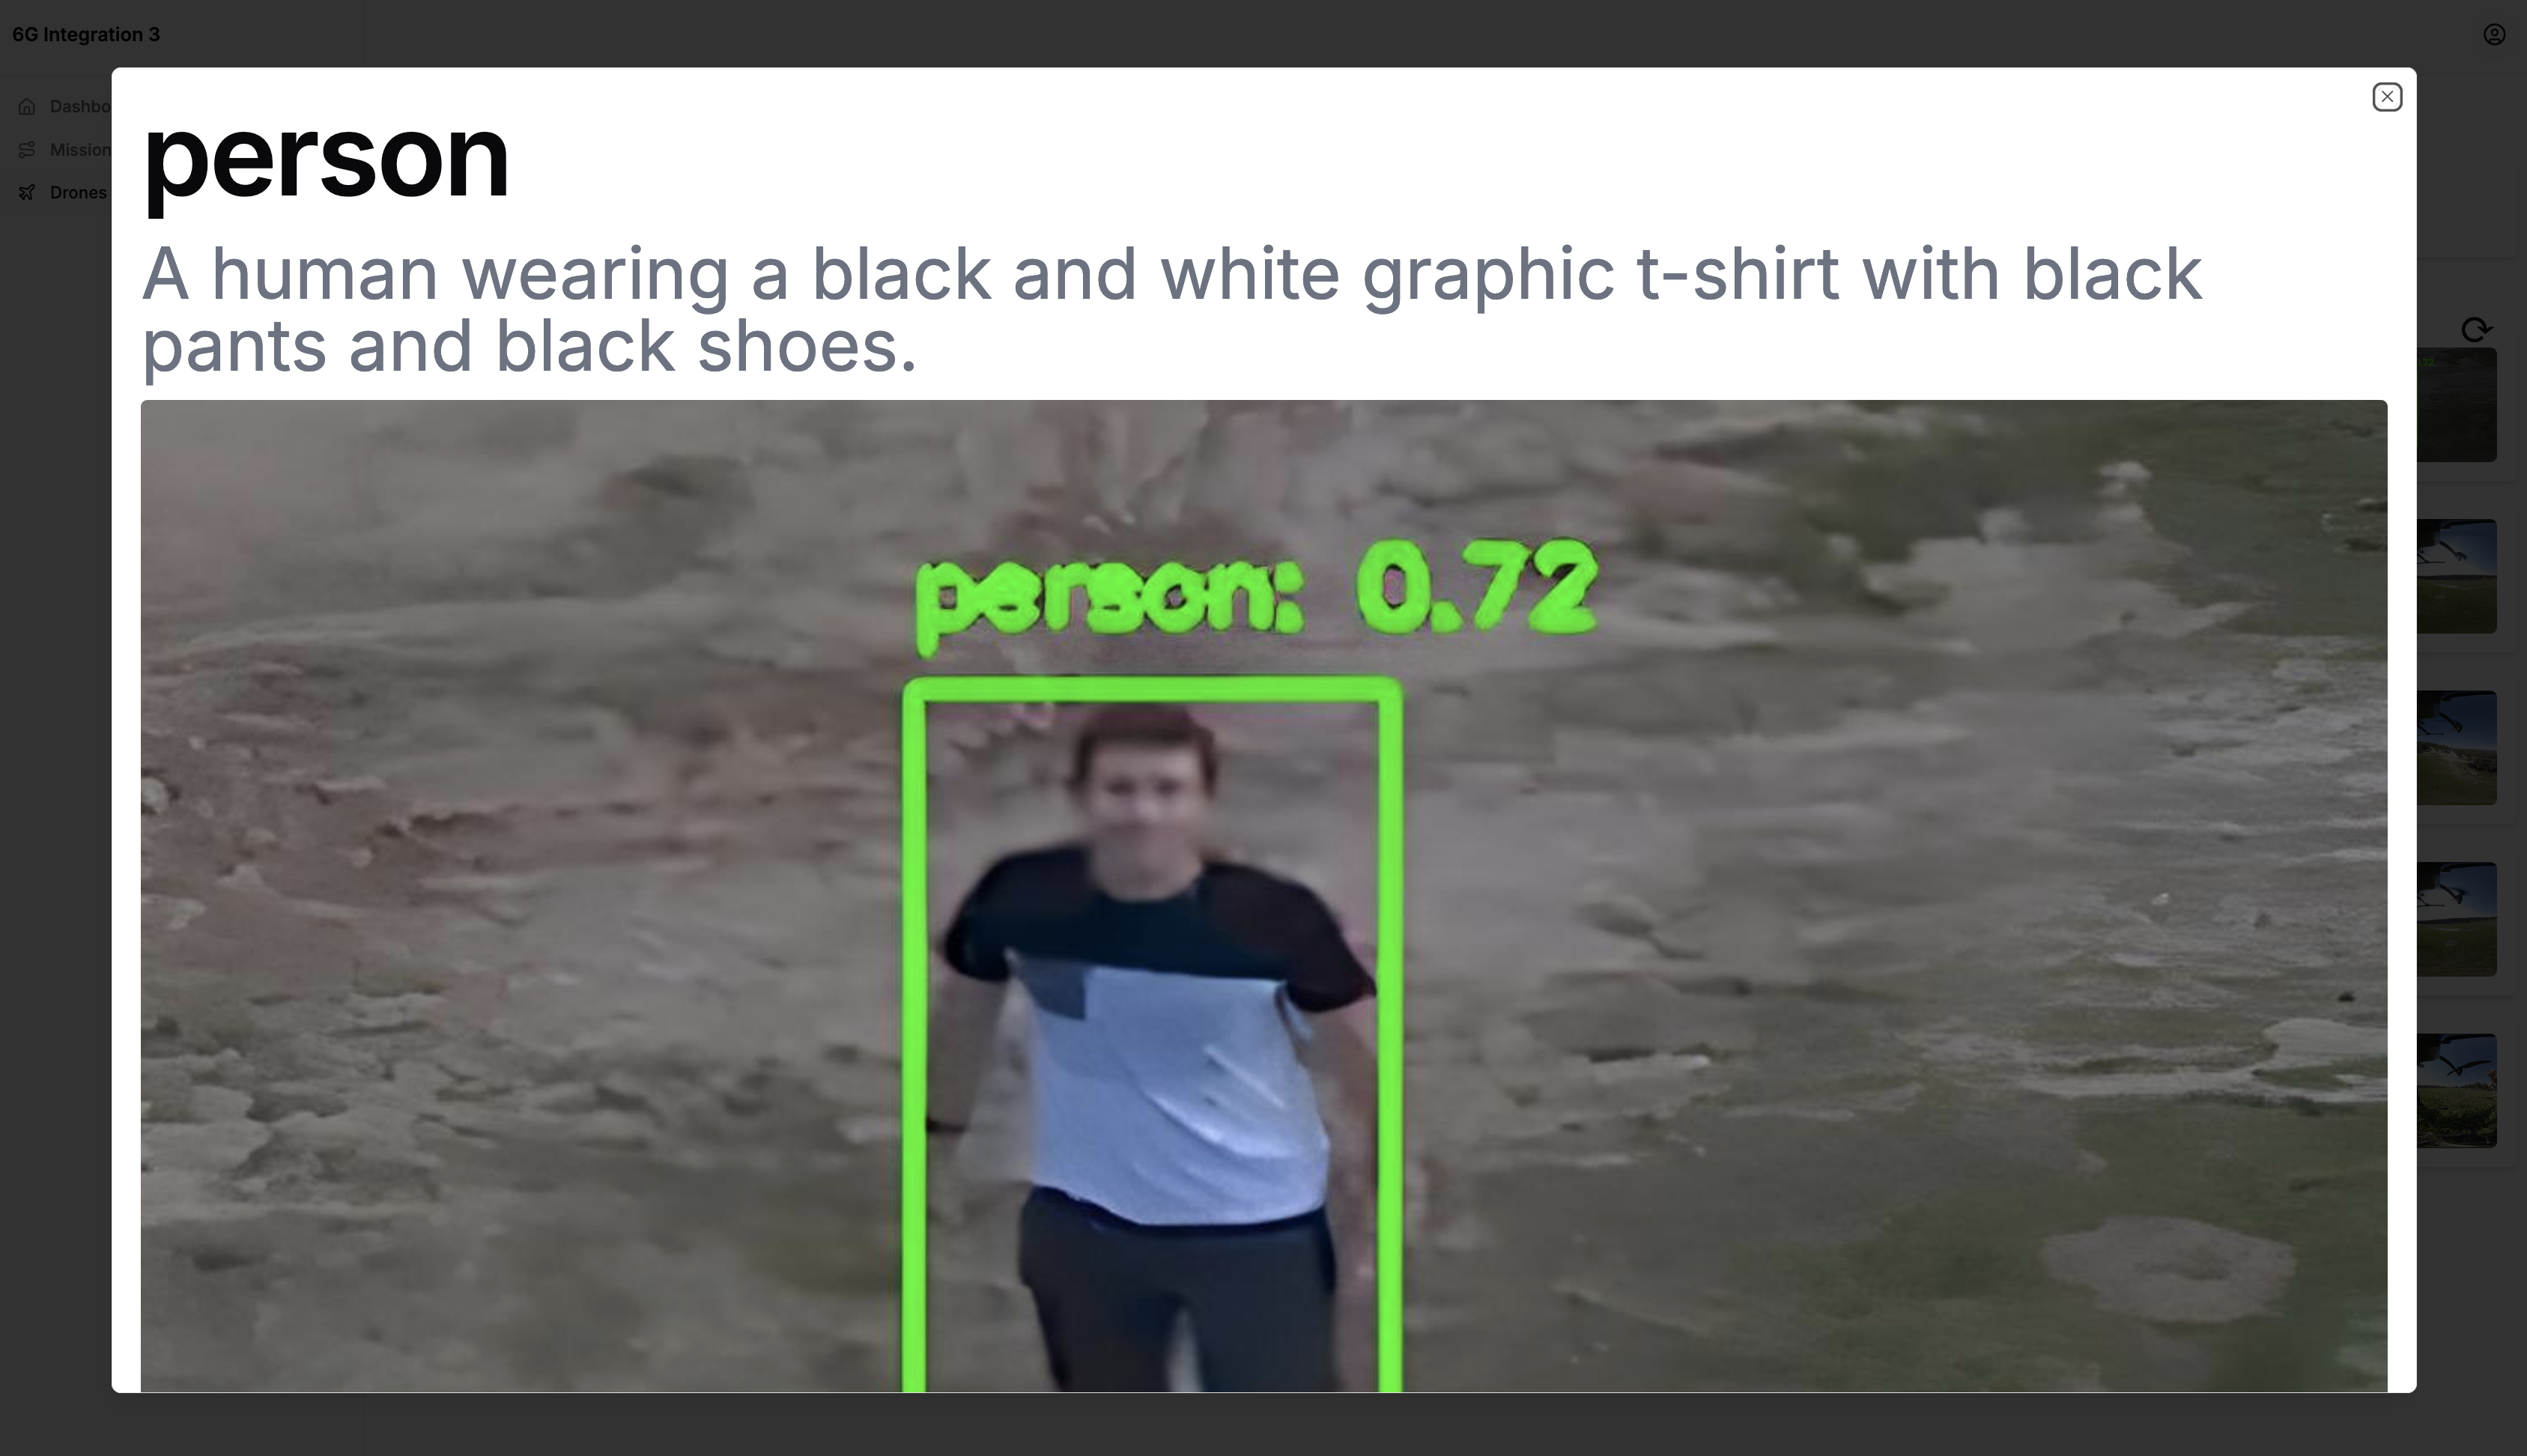
\includegraphics{llm_detection.png}
	\caption{Example of the LLM detection results for a detected object. In this case, the LLM correctly identified the clothes that the person is wearing as the prompt to the image was ``What is the person wearing?''.}\label{fig:llm_detection}
\end{figure}

\subsection{Integration}\label{subsec:implementation_integration}

Finally, all the different components are integrated into the reconnaissance platform to provide a complete processing pipeline to be able to detect the different objects. In \cref{fig:architecture_reconnaissance_platform}, the complete architecture and pipeline can be seen and consists of several interconnected components:

\begin{itemize}
	\item \textbf{Drone Component:} Contains two primary elements:
	      \begin{itemize}
		      \item 360-degree camera for capturing omnidirectional video feed
		      \item Object detection system running directly on the drone for initial processing
	      \end{itemize}
	\item \textbf{VPN Tunnel:} Provides a secure communication channel between the drone and the server infrastructure, ensuring encrypted data transmission.
	\item \textbf{Server Infrastructure:} Comprises two main processing units:
	      \begin{itemize}
		      \item Object Detection module for secondary verification and processing
		      \item Alert system for generating notifications based on detected events
	      \end{itemize}
	\item \textbf{LLM Integration:} The final component in the pipeline that:
	      \begin{itemize}
		      \item Processes detected objects through advanced language models
		      \item Generates contextual insights and natural language descriptions
		      \item Provides enhanced analytical capabilities for operators
	      \end{itemize}
\end{itemize}

The data flow in this architecture follows a sequential pattern where the video feed from the 360-degree camera is first processed locally on the drone for initial object detection. This data is then transmitted through a secure VPN tunnel to the server infrastructure, where it undergoes additional processing and verification. The server component handles both the object detection confirmation and alert generation based on predefined rules and conditions. Finally, the processed data is passed to the LLM integration component, which provides advanced analysis and insights generation for the end-users through the web interface.

This architecture ensures robust security through the VPN tunnel while maintaining efficient data processing and real-time analysis capabilities. The modular design allows for easy scaling and maintenance of individual components without affecting the overall system functionality.

\begin{figure}
	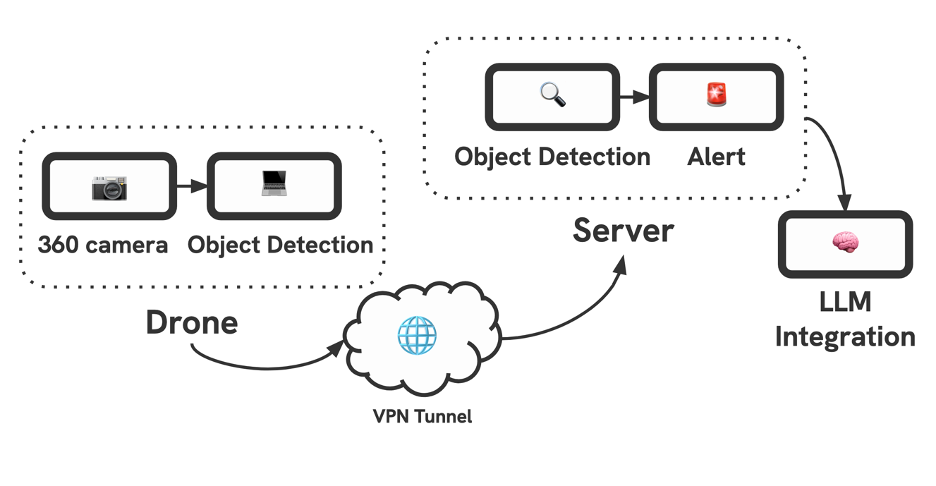
\includegraphics{architecture_reconnaissance_platform.png}
	\caption{Architecture of the reconnaissance platform.} \label{fig:architecture_reconnaissance_platform}
\end{figure}



% Local Variables:
% jinx-local-words: "uav"
% End:
